There are two types of questions in statistical interference:
\begin{itemize}
    \item \textbf{Parameter estimation:} What parameter values would be consistent with the sample data?
    \item \textbf{Hypothesis testing:} Are the sample data consistent with some statement about the parameters?
\end{itemize}

The \begriff{Null Hypothesis} $H_0$ often specifies a single value for the unknown parameter such as "$\alpha = \dots$". It is a default value that can be accepted as holding if there is no evidence against it. A researcher often collects data with the express hope of disapproving the null hypothesis.

If the null hypothesis is not true, we say that the \begriff{alternative hypothesis} $H_A$ holds. If the data are not consistent with the null hypothesis, then we can conclude that the alternative hypothesis must be true. Either the null hypothesis or the alternative hypothesis must be true.

\begin{example}
    The data show the number of operating hours between successive failures of air-conditioning equipment in ten aircrafts. The sample of 199 values is a \begriff{test statistic}. We can test the manufacturer's claim that the rate of failures is no more than one per 110 hours of use.
    \begin{align}
        H_0: \lambda &\le \frac{1}{100}\text{ (claim of a manufacturer)} \notag \\
        H_A: \lambda &> \frac{1}{100} \notag
    \end{align}
    This can be simplified: \\
    \begin{align}
        H_0: \lambda &= \frac{1}{100}\text{ (claim of a manufacturer)} \notag \\
        H_A: \lambda &> \frac{1}{100} \notag
    \end{align}
\end{example}

\subsection{The P-value (Probability value)}

In an industrial process some measurement is normally distributed with standard deviation $\sigma = 10$. Its mean should be $\mu = 520$, but can differ a little bit. Samples of $n=10$ measurements are regularly collected as part of quality control. If a sample had $\bar{x}=529$, does the process need to be adjusted?

\begin{center}
    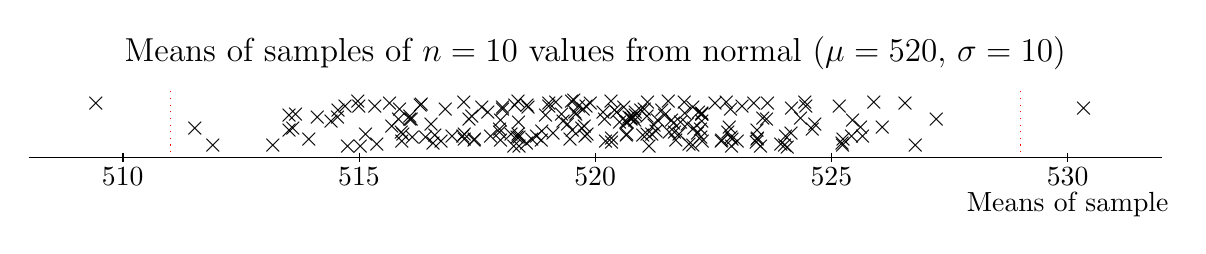
\begin{tikzpicture}[scale=0.6]
		\node at (525.23,0.09) (1) {$\times$};
		\node at (521.10,0.67) (2) {$\times$};
		\node at (519.55,1.00) (3) {$\times$};
		\node at (518.37,0.28) (4) {$\times$};
		\node at (522.27,0.13) (5) {$\times$};
		\node at (522.26,0.55) (6) {$\times$};
		\node at (509.43,0.93) (7) {$\times$};
		\node at (518.28,0.02) (8) {$\times$};
		\node at (522.19,0.74) (9) {$\times$};
		\node at (520.17,0.75) (10) {$\times$};
		\node at (520.22,0.13) (11) {$\times$};
		\node at (519.52,0.37) (12) {$\times$};
		\node at (519.65,0.88) (13) {$\times$};
		\node at (519.50,0.98) (14) {$\times$};
		\node at (515.93,0.28) (15) {$\times$};
		\node at (517.45,0.18) (16) {$\times$};
		\node at (524.65,0.49) (17) {$\times$};
		\node at (520.52,0.54) (18) {$\times$};
		\node at (517.60,0.85) (19) {$\times$};
		\node at (524.15,0.30) (20) {$\times$};
		\node at (521.90,0.73) (21) {$\times$};
		\node at (520.34,0.99) (22) {$\times$};
		\node at (521.04,0.82) (23) {$\times$};
		\node at (525.24,0.06) (24) {$\times$};
		\node at (513.66,0.70) (25) {$\times$};
		\node at (518.39,0.02) (26) {$\times$};
		\node at (520.46,0.76) (27) {$\times$};
		\node at (515.86,0.82) (28) {$\times$};
		\node at (515.90,0.32) (29) {$\times$};
		\node at (519.11,0.31) (30) {$\times$};
		\node at (518.38,0.54) (31) {$\times$};
		\node at (514.55,0.65) (32) {$\times$};
		\node at (524.35,0.63) (33) {$\times$};
		\node at (520.66,0.26) (34) {$\times$};
		\node at (522.26,0.72) (35) {$\times$};
		\node at (519.90,0.94) (36) {$\times$};
		\node at (521.55,0.99) (37) {$\times$};
		\node at (524.03,0.25) (38) {$\times$};
		\node at (521.99,0.07) (39) {$\times$};
		\node at (513.94,0.18) (40) {$\times$};
		\node at (521.20,0.28) (41) {$\times$};
		\node at (524.44,0.97) (42) {$\times$};
		\node at (518.39,0.22) (43) {$\times$};
		\node at (518.56,0.89) (44) {$\times$};
		\node at (518.95,0.69) (45) {$\times$};
		\node at (522.26,0.71) (46) {$\times$};
		\node at (530.34,0.84) (47) {$\times$};
		\node at (516.74,0.13) (48) {$\times$};
		\node at (520.68,0.54) (49) {$\times$};
		\node at (521.57,0.33) (50) {$\times$};
		\node at (523.36,0.93) (51) {$\times$};
		\node at (518.58,0.86) (52) {$\times$};
		\node at (519.83,0.28) (53) {$\times$};
		\node at (519.77,0.45) (54) {$\times$};
		\node at (517.39,0.67) (55) {$\times$};
		\node at (521.89,0.97) (56) {$\times$};
		\node at (514.41,0.56) (57) {$\times$};
		\node at (525.90,0.97) (58) {$\times$};
		\node at (521.62,0.59) (59) {$\times$};
		\node at (523.65,0.93) (60) {$\times$};
		\node at (521.68,0.33) (61) {$\times$};
		\node at (522.09,0.41) (62) {$\times$};
		\node at (519.02,0.88) (63) {$\times$};
		\node at (521.95,0.50) (64) {$\times$};
		\node at (514.71,0.88) (65) {$\times$};
		\node at (521.41,0.79) (66) {$\times$};
		\node at (523.43,0.37) (67) {$\times$};
		\node at (521.81,0.53) (68) {$\times$};
		\node at (521.29,0.34) (69) {$\times$};
		\node at (523.50,0.03) (70) {$\times$};
		\node at (520.85,0.76) (71) {$\times$};
		\node at (522.87,0.82) (72) {$\times$};
		\node at (522.07,0.86) (73) {$\times$};
		\node at (521.25,0.48) (74) {$\times$};
		\node at (521.78,0.28) (75) {$\times$};
		\node at (519.72,0.42) (76) {$\times$};
		\node at (522.24,0.22) (77) {$\times$};
		\node at (515.84,0.61) (78) {$\times$};
		\node at (522.90,0.17) (79) {$\times$};
		\node at (515.03,0.03) (80) {$\times$};
		\node at (520.84,0.59) (81) {$\times$};
		\node at (523.55,0.63) (82) {$\times$};
		\node at (517.79,0.24) (83) {$\times$};
		\node at (520.65,0.54) (84) {$\times$};
		\node at (518.35,0.22) (85) {$\times$};
		\node at (522.88,0.22) (86) {$\times$};
		\node at (514.12,0.65) (87) {$\times$};
		\node at (517.22,0.96) (88) {$\times$};
		\node at (515.34,0.88) (89) {$\times$};
		\node at (511.53,0.42) (90) {$\times$};
		\node at (518.22,0.28) (91) {$\times$};
		\node at (519.59,0.71) (92) {$\times$};
		\node at (522.17,0.31) (93) {$\times$};
		\node at (524.46,0.87) (94) {$\times$};
		\node at (520.20,0.60) (95) {$\times$};
		\node at (518.04,0.86) (96) {$\times$};
		\node at (525.25,0.18) (97) {$\times$};
		\node at (518.30,0.90) (98) {$\times$};
		\node at (517.44,0.16) (99) {$\times$};
		\node at (518.04,0.82) (100) {$\times$};
		\node at (516.83,0.81) (101) {$\times$};
		\node at (522.26,0.70) (102) {$\times$};
		\node at (520.81,0.65) (103) {$\times$};
		\node at (520.61,0.85) (104) {$\times$};
		\node at (522.54,0.95) (105) {$\times$};
		\node at (522.07,0.05) (106) {$\times$};
		\node at (515.14,0.28) (107) {$\times$};
		\node at (521.14,0.04) (108) {$\times$};
		\node at (516.08,0.61) (109) {$\times$};
		\node at (516.57,0.10) (110) {$\times$};
		\node at (525.45,0.59) (111) {$\times$};
		\node at (521.47,0.68) (112) {$\times$};
		\node at (516.13,0.21) (113) {$\times$};
		\node at (518.00,0.16) (114) {$\times$};
		\node at (524.16,0.84) (115) {$\times$};
		\node at (518.87,0.34) (116) {$\times$};
		\node at (515.00,0.88) (117) {$\times$};
		\node at (519.75,0.81) (118) {$\times$};
		\node at (520.41,0.80) (119) {$\times$};
		\node at (522.23,0.39) (120) {$\times$};
		\node at (523.63,0.61) (121) {$\times$};
		\node at (526.56,0.94) (122) {$\times$};
		\node at (521.32,0.58) (123) {$\times$};
		\node at (526.08,0.43) (124) {$\times$};
		\node at (513.60,0.42) (125) {$\times$};
		\node at (520.35,0.19) (126) {$\times$};
		\node at (517.73,0.75) (127) {$\times$};
		\node at (517.23,0.29) (128) {$\times$};
		\node at (517.98,0.38) (129) {$\times$};
		\node at (515.38,0.08) (130) {$\times$};
		\node at (516.11,0.61) (131) {$\times$};
		\node at (513.18,0.06) (132) {$\times$};
		\node at (519.81,0.87) (133) {$\times$};
		\node at (517.20,0.24) (134) {$\times$};
		\node at (520.76,0.62) (135) {$\times$};
		\node at (516.53,0.50) (136) {$\times$};
		\node at (514.76,0.03) (137) {$\times$};
		\node at (513.52,0.68) (138) {$\times$};
		\node at (521.10,0.29) (139) {$\times$};
		\node at (511.91,0.05) (140) {$\times$};
		\node at (519.47,0.18) (141) {$\times$};
		\node at (522.84,0.43) (142) {$\times$};
		\node at (527.22,0.61) (143) {$\times$};
		\node at (525.62,0.44) (144) {$\times$};
		\node at (514.56,0.79) (145) {$\times$};
		\node at (515.91,0.13) (146) {$\times$};
		\node at (521.01,0.26) (147) {$\times$};
		\node at (523.44,0.20) (148) {$\times$};
		\node at (517.98,0.32) (149) {$\times$};
		\node at (515.70,0.45) (150) {$\times$};
		\node at (524.60,0.39) (151) {$\times$};
		\node at (518.86,0.16) (152) {$\times$};
		\node at (518.55,0.09) (153) {$\times$};
		\node at (521.11,0.97) (154) {$\times$};
		\node at (518.76,0.24) (155) {$\times$};
		\node at (519.29,0.70) (156) {$\times$};
		\node at (518.37,0.98) (157) {$\times$};
		\node at (519.79,0.24) (158) {$\times$};
		\node at (520.72,0.65) (159) {$\times$};
		\node at (520.76,0.60) (160) {$\times$};
		\node at (523.01,0.13) (161) {$\times$};
		\node at (523.41,0.12) (162) {$\times$};
		\node at (524.07,0.01) (163) {$\times$};
		\node at (522.68,0.15) (164) {$\times$};
		\node at (521.71,0.15) (165) {$\times$};
		\node at (516.41,0.22) (166) {$\times$};
		\node at (523.11,0.88) (167) {$\times$};
		\node at (523.43,0.18) (168) {$\times$};
		\node at (525.66,0.25) (169) {$\times$};
		\node at (522.78,0.97) (170) {$\times$};
		\node at (513.52,0.37) (171) {$\times$};
		\node at (519.57,0.75) (172) {$\times$};
		\node at (522.67,0.13) (173) {$\times$};
		\node at (520.85,0.69) (174) {$\times$};
		\node at (523.93,0.07) (175) {$\times$};
		\node at (519.32,0.55) (176) {$\times$};
		\node at (520.67,0.29) (177) {$\times$};
		\node at (515.65,0.93) (178) {$\times$};
		\node at (522.89,0.03) (179) {$\times$};
		\node at (519.17,0.96) (180) {$\times$};
		\node at (518.00,0.58) (181) {$\times$};
		\node at (517.23,0.18) (182) {$\times$};
		\node at (526.78,0.05) (183) {$\times$};
		\node at (518.66,0.18) (184) {$\times$};
		\node at (520.97,0.80) (185) {$\times$};
		\node at (516.08,0.67) (186) {$\times$};
		\node at (516.97,0.25) (187) {$\times$};
		\node at (520.35,0.12) (188) {$\times$};
		\node at (516.30,0.90) (189) {$\times$};
		\node at (514.98,0.99) (190) {$\times$};
		\node at (524.01,0.05) (191) {$\times$};
		\node at (517.33,0.60) (192) {$\times$};
		\node at (519.02,0.93) (193) {$\times$};
		\node at (516.61,0.27) (194) {$\times$};
		\node at (525.17,0.87) (195) {$\times$};
		\node at (516.32,0.91) (196) {$\times$};
		\node at (525.43,0.24) (197) {$\times$};
		\node at (522.81,0.33) (198) {$\times$};
		\node at (519.42,0.50) (199) {$\times$};
		\node at (521.66,0.51) (200) {$\times$};
		
		\draw (508,-0.2) -- (532,-0.2);
		\draw (510,-0.1) -- (510,-0.3);
		\node at (510,-0.6) (510) {510};
		\draw (515,-0.1) -- (515,-0.3);
		\node at (515,-0.6) (515) {515};
		\draw (520,-0.1) -- (520,-0.3);
		\node at (520,-0.6) (520) {520};
		\draw (525,-0.1) -- (525,-0.3);
		\node at (525,-0.6) (525) {525};
		\draw (530,-0.1) -- (530,-0.3);
		\node at (530,-0.6) (530) {530};
		
		\draw[red,dotted] (511,1.2) -- (511,-0.2);
		\draw[red,dotted] (529,1.2) -- (529,-0.2);
		
		\node at (530,-1.2) (axis) {Means of sample};
		\node at (520,2) (top) {\large Means of samples of $n=10$ values from normal ($\mu=520$, $\sigma=10$)};
	\end{tikzpicture}
\end{center}

From the 200 simulated samples above (\person{Monte Carlo} simulation), it seems very unlikely that a sample mean of 529 would have been recorded if $\mu = 529$. There is strong evidence that the industrial process no longer has a mean of $\mu = 520$ and needs to be adjusted.

\begin{definition}[p-value]
    A \begriff{p-value} describes the \textbf{evidence against} $H_0$. A p-value is evaluated from a random sample so it has a distribution in the same way that a sample mean has a distribution.
\end{definition}

\begin{center}
    \begin{tabular}{p{4cm}|p{7cm}}
        \textbf{p-value} & \textbf{Interpretation} \\
        \hline
        over 0.1 & no evidence that $H_0$ does not hold \\
        between 0.05 and 0.1 & very weak evidence that $H_0$ does not hold \\
        between 0.01 and 0.05 & moderately strong evidence that $H_0$ does not hold \\
        under 0.01 & strong evidence that $H_0$ does not hold
    \end{tabular}
\end{center}

\begin{example}[normal distribution with known $\sigma$, one-tailed test]
    We are given a random sample of $n=30$ with $\bar{x}=16.8$. Does the population have mean $\mu=18.3$ and standard deviation $\sigma=7.1$, or is the mean now lower than 18.3?
    \begin{align}
        H_0: \mu &= 18.3 \notag \\
        H_A: \mu &< 18.3 \notag
    \end{align}
    The p-value can be evaluated using the statistical distance of 16.8 from 18.3 (a z statistic).
    \begin{align}
        z = \frac{\bar{x} - 18.3}{\underbrace{\frac{7.1}{\sqrt{30}}}_{\text{standard error}}} = -1.157 \notag
    \end{align}
    \begin{center}
    \begin{tikzpicture}
            \begin{axis}[
		    xmin=-3, xmax=3, xlabel=$z$,
		    ymin=0, ymax=0.6,
		    samples=400,
		    axis y line=middle,
		    axis x line=middle,
		    ]
		    \addplot[name path=f,blue] {1/(sqrt(2*pi))*exp(-0.5*x^2)};
		    \path[name path=axis] (axis cs:-3,0) -- (axis cs:-1.157,0);
		    \addplot [thick,color=blue,fill=blue,fill opacity=0.3] fill between[of=f and axis,soft clip={domain=-3:-1.157},];
		    \draw [dotted] (axis cs:-1.157,0) -- (axis cs:-1.157,0.6);
		    \node at (axis cs:-2.5,0.25) (node) {p-value};
		    \draw (axis cs:-2.5,0.23) -- (axis cs:-1.5,0.08);
		    \end{axis}
    \end{tikzpicture}
    \end{center}
    \begin{align}
        \text{p-value} = P(z \le -1.157) = 0.124 \notag
    \end{align}
    The p-value is reasonably large, meaning that a sample mean as low as 16.8 would not be unusual if $\mu=18.3$, so there is no evidence against $H_0$.
\end{example}

\begin{*anmerkung}
	To compute the p-value you can use
	\begin{align}
		\text{p-value} = \texttt{CDF(NormalDistribution(0,1),-1.157)}\notag
	\end{align}
\end{*anmerkung}

\begin{example}[normal distribution with known $\sigma$, two-tailed test]
    Companies test their products to ensure that the amount of active ingredient is within some limits. However the chemical analysis is not precise and repeated measurements of the same specimen usually differ slightly. One type of analysis gives results that are normally distributed with a mean that depend on the actual product being tested and standard deviation 0.0068 grams per litre. A product is tested three times with the following concentrations of the active ingredient: 0.8403, 0.8363, 0.8447 grams per litre. are the data consistent with the target concentration of 0.85 grams per litre?
    \begin{center}
       \begin{tabular}{p{4cm}|p{7cm}}
            null hypothesis & $H_0$: $\mu=0.85$ \\
            \hline
            alternative hypothesis & $H_A$: $\mu\neq 0.85$ \\
            \hline
            test statistic & $\bar{x} = 0.8404$, $z=\frac{0.8404-0.85}{\frac{0.0068}{\sqrt{3}}} = -2.437$, $P(z\le -2.437) = 0.00741$ \\
            \hline
            p-value & $2\cdot 0.00741 = 0.0148$ \\
            \hline
            p-value interpretation & There is moderately strong evidence that the true concentration is not 0.85.
       \end{tabular}
    \end{center}
	\begin{center}
		\begin{tikzpicture}
			\begin{axis}[
				xmin=-3, xmax=3, xlabel=$z$,
				ymin=0, ymax=0.6,
				samples=400,
				axis y line=middle,
				axis x line=middle,
				]
				\addplot[name path=f,blue] {1/(sqrt(2*pi))*exp(-0.5*x^2)};
				\path[name path=axis] (axis cs:-3,0) -- (axis cs:-2.437,0);
				\path[name path=axis2] (axis cs:2.437,0) -- (axis cs:3,0);
				\addplot [thick,color=blue,fill=blue,fill opacity=0.3] fill between[of=f and axis,soft clip={domain=-3:-2.437},];
				\addplot [thick,color=blue,fill=blue,fill opacity=0.3] fill between[of=f and axis2,soft clip={domain=2.437:3},];
				\draw [dotted] (axis cs:-2.437,0) -- (axis cs:-2.437,0.6);
				\draw [dotted] (axis cs:2.437,0) -- (axis cs:2.437,0.6);
				\node at (axis cs:-1.5,0.25) (node) {p-value};
				\draw (axis cs:-1.7,0.23) -- (axis cs:-2.7,0.002);
				\draw (axis cs:-1.3,0.23) -- (axis cs:2.7,0.002);
			\end{axis}
		\end{tikzpicture}
	\end{center}
\end{example}

\begin{example}[normal distribution with unknown $\sigma$, one-tailed test]
    Both cholesterol and saturated fats are often avoided by people who are trying to lose weight or reduce their blood cholesterol level. Cooking oil made from soybeans has little cholesterol and has been claimed to have only 15\% saturated fat. A clinician believes that the saturated fat content is greater than 15\% and randomly samples 13 bottles of soybean cooking oil for testing with the following percentage saturated fat: 15.2, 12.4, 15.4, 13.5, 15.9, 17.1, 16.9, 14.3, 19.1, 18.2, 15.5, 16.3, 20.0.
    \begin{center}
       \begin{tabular}{p{4cm}|p{7cm}}
            null hypothesis & $H_0$: $\mu=15$ \\
            \hline
            alternative hypothesis & $H_A$: $\mu > 15$ \\
            \hline
            T-test for $\mu$ & $\bar{x} = 16.138$, $t=\frac{16.138-15}{\frac{2.154}{\sqrt{13}}} = 1.906$, $P(t\ge 1.906) = 0.040$ (t-distribution with 12 degrees of freedom) \\
            \hline
            p-value interpretation & Since this is below 0.05, we conclude that there is moderately strong evidence that the mean saturated fat content of the oils is higher than the claimed 15\%.
       \end{tabular}
    \end{center}
	\begin{center}
		 \begin{tikzpicture}
			\begin{axis}[
				xmin=-3, xmax=3, xlabel=$z$,
				ymin=0, ymax=0.6,
				samples=400,
				axis y line=middle,
				axis x line=middle,
				]
				\addplot[name path=f,blue] {4041576*(1/(x^2 + 12))^(13/2)};
				\path[name path=axis] (axis cs:-3,0) -- (axis cs:-1.906,0);
				\addplot [thick,color=blue,fill=blue,fill opacity=0.3] fill between[of=f and axis,soft clip={domain=-3:-1.906},];
				\draw [dotted] (axis cs:-1.906,0) -- (axis cs:-1.906,0.6);
				\node at (axis cs:-2.5,0.25) (node) {p-value};
				\draw (axis cs:-2.5,0.23) -- (axis cs:-2.2,0.03);
			\end{axis}
		\end{tikzpicture}
	\end{center}
\end{example}

A hypothesis test is based on two competing hypotheses about the value of a parameter $\theta$. \\
Null hypothesis $H_0$: $\theta = \theta_0$ \\
Alternative hypothesis (one-tailed test) $H_A$: $\theta > \theta_0$

The hypothesis test is based on a test statistic that is some function of the data values:
\begin{align}
    Q = g(x_1,...,x_n\vert\theta_0) \notag
\end{align}
whose distribution is fully known when $H_0$ is true (i.e. when $\theta_0$ is the true parameter value). We evaluate the test statistic to assess whether it is unusual enough to throw doubt on the null hypothesis.

\begin{center}
    \begin{tikzpicture}
            \begin{axis}[
		    xmin=0, xmax=4,
		    ymin=0, ymax=1,
		    samples=400,
		    axis y line=middle,
		    axis x line=middle,
		    restrict y to domain=0:1,
		    ]
		    \addplot[name path=f,blue] {1/(x*sqrt(2*pi))*exp(-0.5*(ln(x))^2)};
		    \path[name path=axis] (axis cs:2,0) -- (axis cs:4,0);
		    \addplot [thick,color=blue,fill=blue,fill opacity=0.3] fill between[of=f and axis,soft clip={domain=2:4}];
		    \draw [dotted] (axis cs:2,0) -- (axis cs:2,0.55);
		    \node at (axis cs:3,0.5) (1) {observed value of $Q$};
		    \node at (axis cs:1.7,0.75) (2) {distribution of $Q$ when $H_0$ is true};
		    \node at (axis cs:3,0.3) (3) {p-value};
		    \draw (axis cs:3,0.25) -- (axis cs:2.5,0.05);
		    \end{axis}
        \end{tikzpicture}
\end{center}

\begin{theorem}
    P-values close to zero throw doubt on the null hypothesis.
\end{theorem}

\subsection{The significance level}

\begin{definition}[significance level]
    The \begriff{significance level} is the probability of wrongly concluding that $H_0$ does not hold when it actually does.
\end{definition}

\begin{itemize}
    \item \textbf{One-tailed test:} For example, it may be acceptable to have a 5\% chance of concluding that $\theta<\theta_0$ when actually $\theta=\theta_0$. This means a significance level (tail area of the test statistic's distribution) of this test is $\alpha=0.05$.
    \item \textbf{Two-tailed test:} Values at both tails of the distribution of the test statistic result in rejection of $H_0$, so the corresponding tail areas should each have area $\frac{\alpha}{2}$ for a test with significance level $\alpha$.
\end{itemize}

\begin{example}
    Cooking oil made from soybeans has little cholesterol and has been claimed to have only 15\% saturated fat. A clinician believes that the saturated fat content is greater than 15\% and randomly samples 13 bottles of soybean cooking oil for testing: 15.2, 12.4, 15.4, 13.5, 15.9, 17.1, 16.9, 14.3, 19.1, 18.2, 15.5, 16.3, 20.0.
    \begin{center}
        \begin{tabular}{p{4cm}|p{7cm}}
        Null hypothesis & $H_0$: $\mu=15$ \\
        \hline
        Alternative hypothesis & $H_A$: $\mu > 15$ \\
        \hline
        \multicolumn{2}{p{11cm}}{A significance level of $\alpha=0.05$ means that the clinician is willing to wrongly conclude that the saturated fat content is over 15\% when it really is 15\% with probability 0.05.} \\
        \hline
        t-statistic & $t=\frac{\bar{x}-15}{\frac{s}{\sqrt{13}}} = 1.906$ \\
        \hline
        rejection region & $P(T>1.782) = 0.05$ (t distribution with 12 degrees of freedom) \\
        \hline
        Conclusion & $t$ lies in the rejection region so $H_0$ is rejected at the 5\% significance level.
    \end{tabular}
    \end{center}
	\begin{center}
		\begin{tikzpicture}
		\begin{axis}[
		xmin=-3, xmax=3, xlabel=$x$,
		ymin=0, ymax=1, ylabel=$y$,
		samples=400,
		axis y line=middle,
		axis x line=middle,
		domain=-3:3,
		restrict y to domain=0:1,
		width = 16cm,
		height = 8cm,
		]
		\addplot[name path=f,blue] {4041576/((x^2+12)^(6.5))};
		\path[name path=axis] (axis cs:1.782,0) -- (axis cs:3,0);
		\draw (axis cs:1.782,0) -- (axis cs:1.782,1);
		\draw [dotted] (axis cs:1.906,0) -- (axis cs:1.906,0.6);
		\node at (axis cs:1,0.5) (a) {0.05};
		\draw (axis cs:1, 0.46) -- (axis cs: 2.2,0.02);
		\node at (axis cs: 2.0,0.95) (b) {1.782};
		\node at (axis cs: 2.1,0.55) (c) {1.906};
		\node[red] at (axis cs: 2.4,0.78) (d) {rejection region};
		\begin{scope}[transparency group]
		\begin{scope}[blend mode=multiply]
			\addplot [thick,color=blue,fill=blue,fill opacity=0.3] fill between[of=f and axis,soft clip={domain=1.782:3},];
			\draw[red,fill=red,opacity=0.2] (axis cs: 1.782,0) -- (axis cs: 1.782,1) -- (axis cs: 3,1) -- (axis cs: 3,0) -- (axis cs: 1.782,0);
		\end{scope}
		\end{scope}
		\end{axis}
		\end{tikzpicture}
	\end{center}
\end{example}

\begin{definition}[Type 1 + 2 error]
    The \begriff{Type 1 error} is the significance level of the test. The decision rule is usually defined to make the significance level 5\% or 1\%.
    
    The \begriff{Type 2 error} is wrongly accepting $H_0$ when it is false.
\end{definition}

Instead of the probability of a Type 2 error, it is common to use the \begriff{power} of a test, defined as one minus the probability of a Type 2 error. The power of a test is the probability of correctly rejecting $H_0$ when it is false.
\begin{center}
    \begin{tabular}{p{2cm}p{2cm}|p{3cm}|p{3cm}}
     & & \multicolumn{2}{|c}{Decision} \\
     \cline{3-4}
     & & accept $H_0$ & reject $H_0$ \\
     \hline
     \multirow{3}{*}{Truth} & \multicolumn{1}{|l|}{$H_0$ is true} & \cellcolor{green} & \cellcolor{red}significance level = P(Type 1 error) \\
     \cline{2-4}
     & \multicolumn{1}{|l|}{$H_0$ is false} & \cellcolor{red}$P(\text{Type 2 error})$ & \cellcolor{green}Power = 1 - P(Type 2 error) \\
\end{tabular}
\end{center}

Computer software can provide the p-value for a hypothesis test at 5\% or 1\% significance level (Type 1 error).

It is clearly desirable to use a test whose power is as close to 1 as possible. There are three different ways to increase the power:
\begin{itemize}
    \item \textbf{Increase the significance level:} If the critical value for the test is adjusted, increasing the probability of a Type 1 error decreases the probability of a Type 2 error and therefore increase the power.
    \item \textbf{Use a different decision rule:} For example, in a test about the mean of a normal population, a decision rule based on the sample median has lower power than a decision rule based on the sample mean.
    \item \textbf{Increase the sample size:} By increasing the amount of data on which we base our decision about whether to accept or reject $H_0$, the probabilities of making errors can be reduced.
\end{itemize}

When the significance level is fixed, increasing the sample size is therefore usually the only way to improve the power.

Ideally there should be a trade-off between low significance level (Type 1 error) and high power. The desired power of the test is usually 0.8. The power of a test is not a single value since the alternative hypothesis allows for a range of different parameter values. It is represented by a power function that can be graphed against the possible parameter values. MATLAB \texttt{sampsizepwr} can compute the sample size to obtain a particular power for a hypothesis test, given the parameter value of the alternative hypothesis.

\begin{center}
    	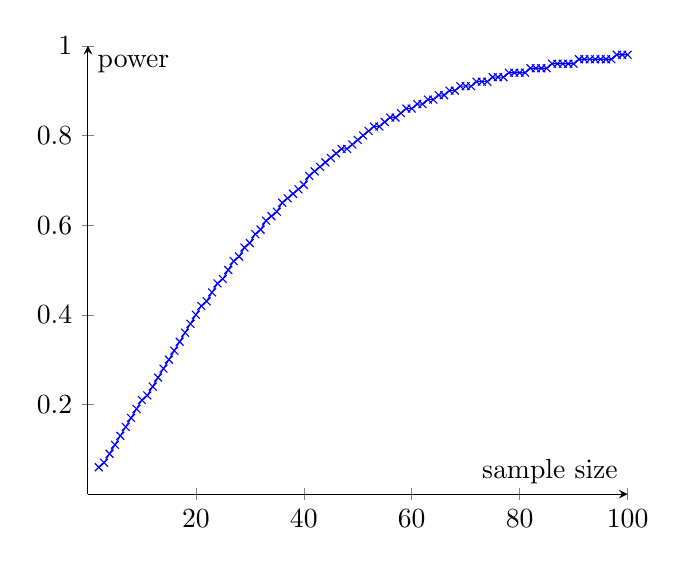
\begin{tikzpicture}
		\begin{axis}[
		xmin=0, xmax=100, xlabel=sample size,
		ymin=0, ymax=1, ylabel=power,
		samples=401,
		axis y line=middle,
		axis x line=middle,
		restrict y to domain=0:1,
		]
		\addplot[mark=x, blue] coordinates {
			(  2,0.06)
			(  3,0.07)
			(  4,0.09)
			(  5,0.11)
			(  6,0.13)
			(  7,0.15)
			(  8,0.17)
			(  9,0.19)
			( 10,0.21)
			( 11,0.22)
			( 12,0.24)
			( 13,0.26)
			( 14,0.28)
			( 15,0.30)
			( 16,0.32)
			( 17,0.34)
			( 18,0.36)
			( 19,0.38)
			( 20,0.40)
			( 21,0.42)
			( 22,0.43)
			( 23,0.45)
			( 24,0.47)
			( 25,0.48)
			( 26,0.50)
			( 27,0.52)
			( 28,0.53)
			( 29,0.55)
			( 30,0.56)
			( 31,0.58)
			( 32,0.59)
			( 33,0.61)
			( 34,0.62)
			( 35,0.63)
			( 36,0.65)
			( 37,0.66)
			( 38,0.67)
			( 39,0.68)
			( 40,0.69)
			( 41,0.71)
			( 42,0.72)
			( 43,0.73)
			( 44,0.74)
			( 45,0.75)
			( 46,0.76)
			( 47,0.77)
			( 48,0.77)
			( 49,0.78)
			( 50,0.79)
			( 51,0.80)
			( 52,0.81)
			( 53,0.82)
			( 54,0.82)
			( 55,0.83)
			( 56,0.84)
			( 57,0.84)
			( 58,0.85)
			( 59,0.86)
			( 60,0.86)
			( 61,0.87)
			( 62,0.87)
			( 63,0.88)
			( 64,0.88)
			( 65,0.89)
			( 66,0.89)
			( 67,0.90)
			( 68,0.90)
			( 69,0.91)
			( 70,0.91)
			( 71,0.91)
			( 72,0.92)
			( 73,0.92)
			( 74,0.92)
			( 75,0.93)
			( 76,0.93)
			( 77,0.93)
			( 78,0.94)
			( 79,0.94)
			( 80,0.94)
			( 81,0.94)
			( 82,0.95)
			( 83,0.95)
			( 84,0.95)
			( 85,0.95)
			( 86,0.96)
			( 87,0.96)
			( 88,0.96)
			( 89,0.96)
			( 90,0.96)
			( 91,0.97)
			( 92,0.97)
			( 93,0.97)
			( 94,0.97)
			( 95,0.97)
			( 96,0.97)
			( 97,0.97)
			( 98,0.98)
			( 99,0.98)
			(100,0.98)
		};
		\end{axis}
		\end{tikzpicture}
\end{center}

There are a many number of statistical tests for assessing normality: \person{Shapiro-Wilk} test, \person{Kolmogorov-Smirnov} test, \person{Jacque-Bera} test, etc. The \person{Shapiro-Wilk} test ($n<50$) can be used to verify whether data come from a normal distribution: \\
$H_0$: sample data are not significantly different than a normal population. \\
$H_A$: sample data are significantly different than a normal population. \\
P-value $>0.05$ mean the data are normal \\
P-value $<0.05$ mean the data are not normal \\
\person{Monte Carlo} simulations proved the efficiency of \person{Shapiro-Wilk} test. It s preferable that normality is assessed visually as well! The \person{Kolmogorov-Smirnov} non-parametric test ($n>50$) examines if scores are likely to follow some distribution in some population (not necessarily normal).